\chapter{smartphone}
\label{ch:smartphone}

\section*{Introduction}

Dans votre poche se trouve un appareil qui a changé la vie de milliards de personnes partout dans le monde. Le troisième écran personnel (après la télévision et l’ordinateur) est le plus personnelle de tous et  est la priorité clés des entreprises de cette décenies afin de proposer de nouveaux services.

Cependant le développement mobile est une activité plus difficile que le développement sur Pc. Les plateformes mobles sont très fragmentés et les développeurs doivent travailler avec un minumum de ressources. Heureusement le web-mobile permet de traiter plus facilement cette fragmentation en permettant aux développeurs de créer des applications qui s’éxecutent sur plus de plates-formes qu’en natif.

Les statistiques les plus récentes au moment de la rédaction de ce mémoire indique que Android est en tête du classement des smartphones avec environ de 70% de toutes les ventes au dernier trimestres 2012, iOS est à environ 20% dans la même période. Blackberry un très grand nom dans le monde des smartphone a moins de 10%, tandis que Windows Phone, Bada et Symbian avec d’autre plateformes plus ou moins connus, ont partagé le reste des pourcentages restant.


\begin{center}
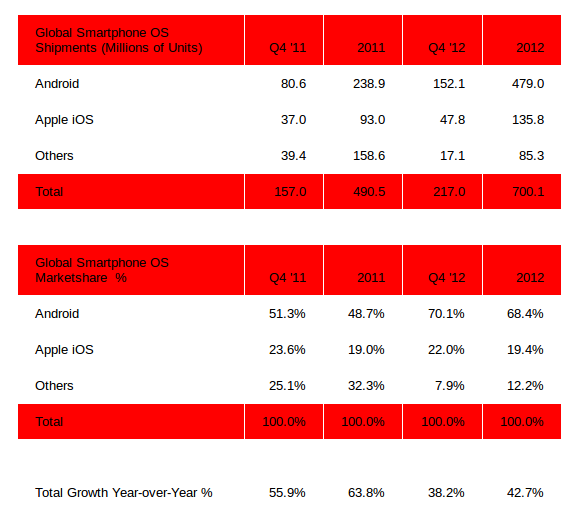
\includegraphics[width=14cm]{img/marche_smartphone.png}
\label{Parts de marché smartphone  }
\end{center}

Ces chiffres montrent clairement que le marché des smartphones est très différent du marché du marché des PC, il n’y a pas vraiment de gagnant et les societés voulant profiter dece nouveau canal de communication ont à faire d’importants investissement afin d’être présents dans autant de poches que possible. Beaucoup d’applications doivent être écrite dans au moins deux ou trois plates-fomres (généralement iOS, Android et Blackberry) pour atteindre une tranche non négligeable du marché.

Actuellement les smartphone ont conquéri le marché des téléphones portables ces dernières années.

Beaucoup de choses ont changé depuis 2007, mais comme comme pour son homologue de bureau, le Web apparaît comme la solution multiplateforme la plus importante à la dispositions des développeurs d’aujourd’hui.
La croissance du Web mobiles

Une des avancées de cette nouvelle génération d’appareils mobiles est la disponibilité d’utiliser pleinement un véritable navigateur Web mobiles, compatible avec la plupart des normes actuelles telles que HTML5, CSS, JavaScript et de nombreux autres standard.

Beaucoup d’entre nous se souviennent regarder Steve Jobs présentant les capacités du navigateur Safari mobile dans le premier iPhone, tout en reconnaissant qu’une nouvelle ère avait commencé précisément ce jour-là.

Les navigateurs mobiles ne doivent pas seulement être aussi capable que leurs homologues de bureau, ils étaient meilleurs que les pc , ils étaient rapide et étaient entièrement conformes aux normes.

La montée en puissance de l’internet mobile a apporté de nouvelles possibilités, en particulier dans les pays à faibles pénétration technologique comme l’Amérique latine ou l’Afrique. Les smartphone apparaissent alors comme un bien beaucoup moins cher pour accéder aux informations et services en ligne.

Exemple, en 2010, plus de 30% de tout les accès web à partir de l’Afrique était fait à partir d’un smartphone.

Dans le monde, on estime que plus de 50% de tout les requêtes web viendront d’appareils mobile d’ici 2015.

Nouveaux paradigmes

Tout cela représente un énorme changement dans nos habitudes de développer des logiciels.

Un changement radical indiquant  que le web mobile est en train de devenir le nouveau canal principal de la présence du web. L’utilisation de la bande passante à partir d’un pc va être inférieur à celle du mobile.

Mais cette nouvelle perspective pose quelques questions:

        Combien de plateforme je dois tester pour mon site web?

        Dois-je me soucier des téléphones mobiles bas de gamme?

        Quel bibliothèques puis-je utiliser pour accélérer mon développement?

        Quel est le niveau de support des standard dans les principaux navigateurs mobiles.

Pour ce faire, nous allons étudier les dans les technologies suivantes, qui sont actuellement très prometteuses et qui ont une feuillent de route très interessantes

    PhoneGap

    Sencha Touch

    Jquery Mobile


Il y’a bien sur d’autre technologies interessantes mais je vais me limiter à l’étude de ces 3 frameworks.


